\documentclass{standalone} 

%\documentclass[a0]{sciposter}
\usepackage[T1]{fontenc}
\usepackage[latin1]{inputenc}
%\usepackage[margin=-1in]{geometry}
\usepackage[centertags]{amsmath}
\usepackage{amsfonts,multicol}
\usepackage{graphicx,colortbl}
\usepackage{amsmath,amsfonts,amssymb}
\usepackage{hyperref}
\hypersetup{pdfpagelayout=SinglePage}

\pagestyle{plain}

\newcommand{\pcsize}{28}
\newcommand{\tapeSize}{30}
\newcommand{\sewOverlap}{.5}

\newcommand{\pcrad}{({\pcsize/2} )}
\newcommand{\pcRadOver}{{(\pcsize/2 + \sewOverlap)}}
\newcommand{\MpcRadOver}{{-(\pcsize/2 + \sewOverlap)}}
\usepackage{verbatim}
\usepackage{tikz}
\begin{document}

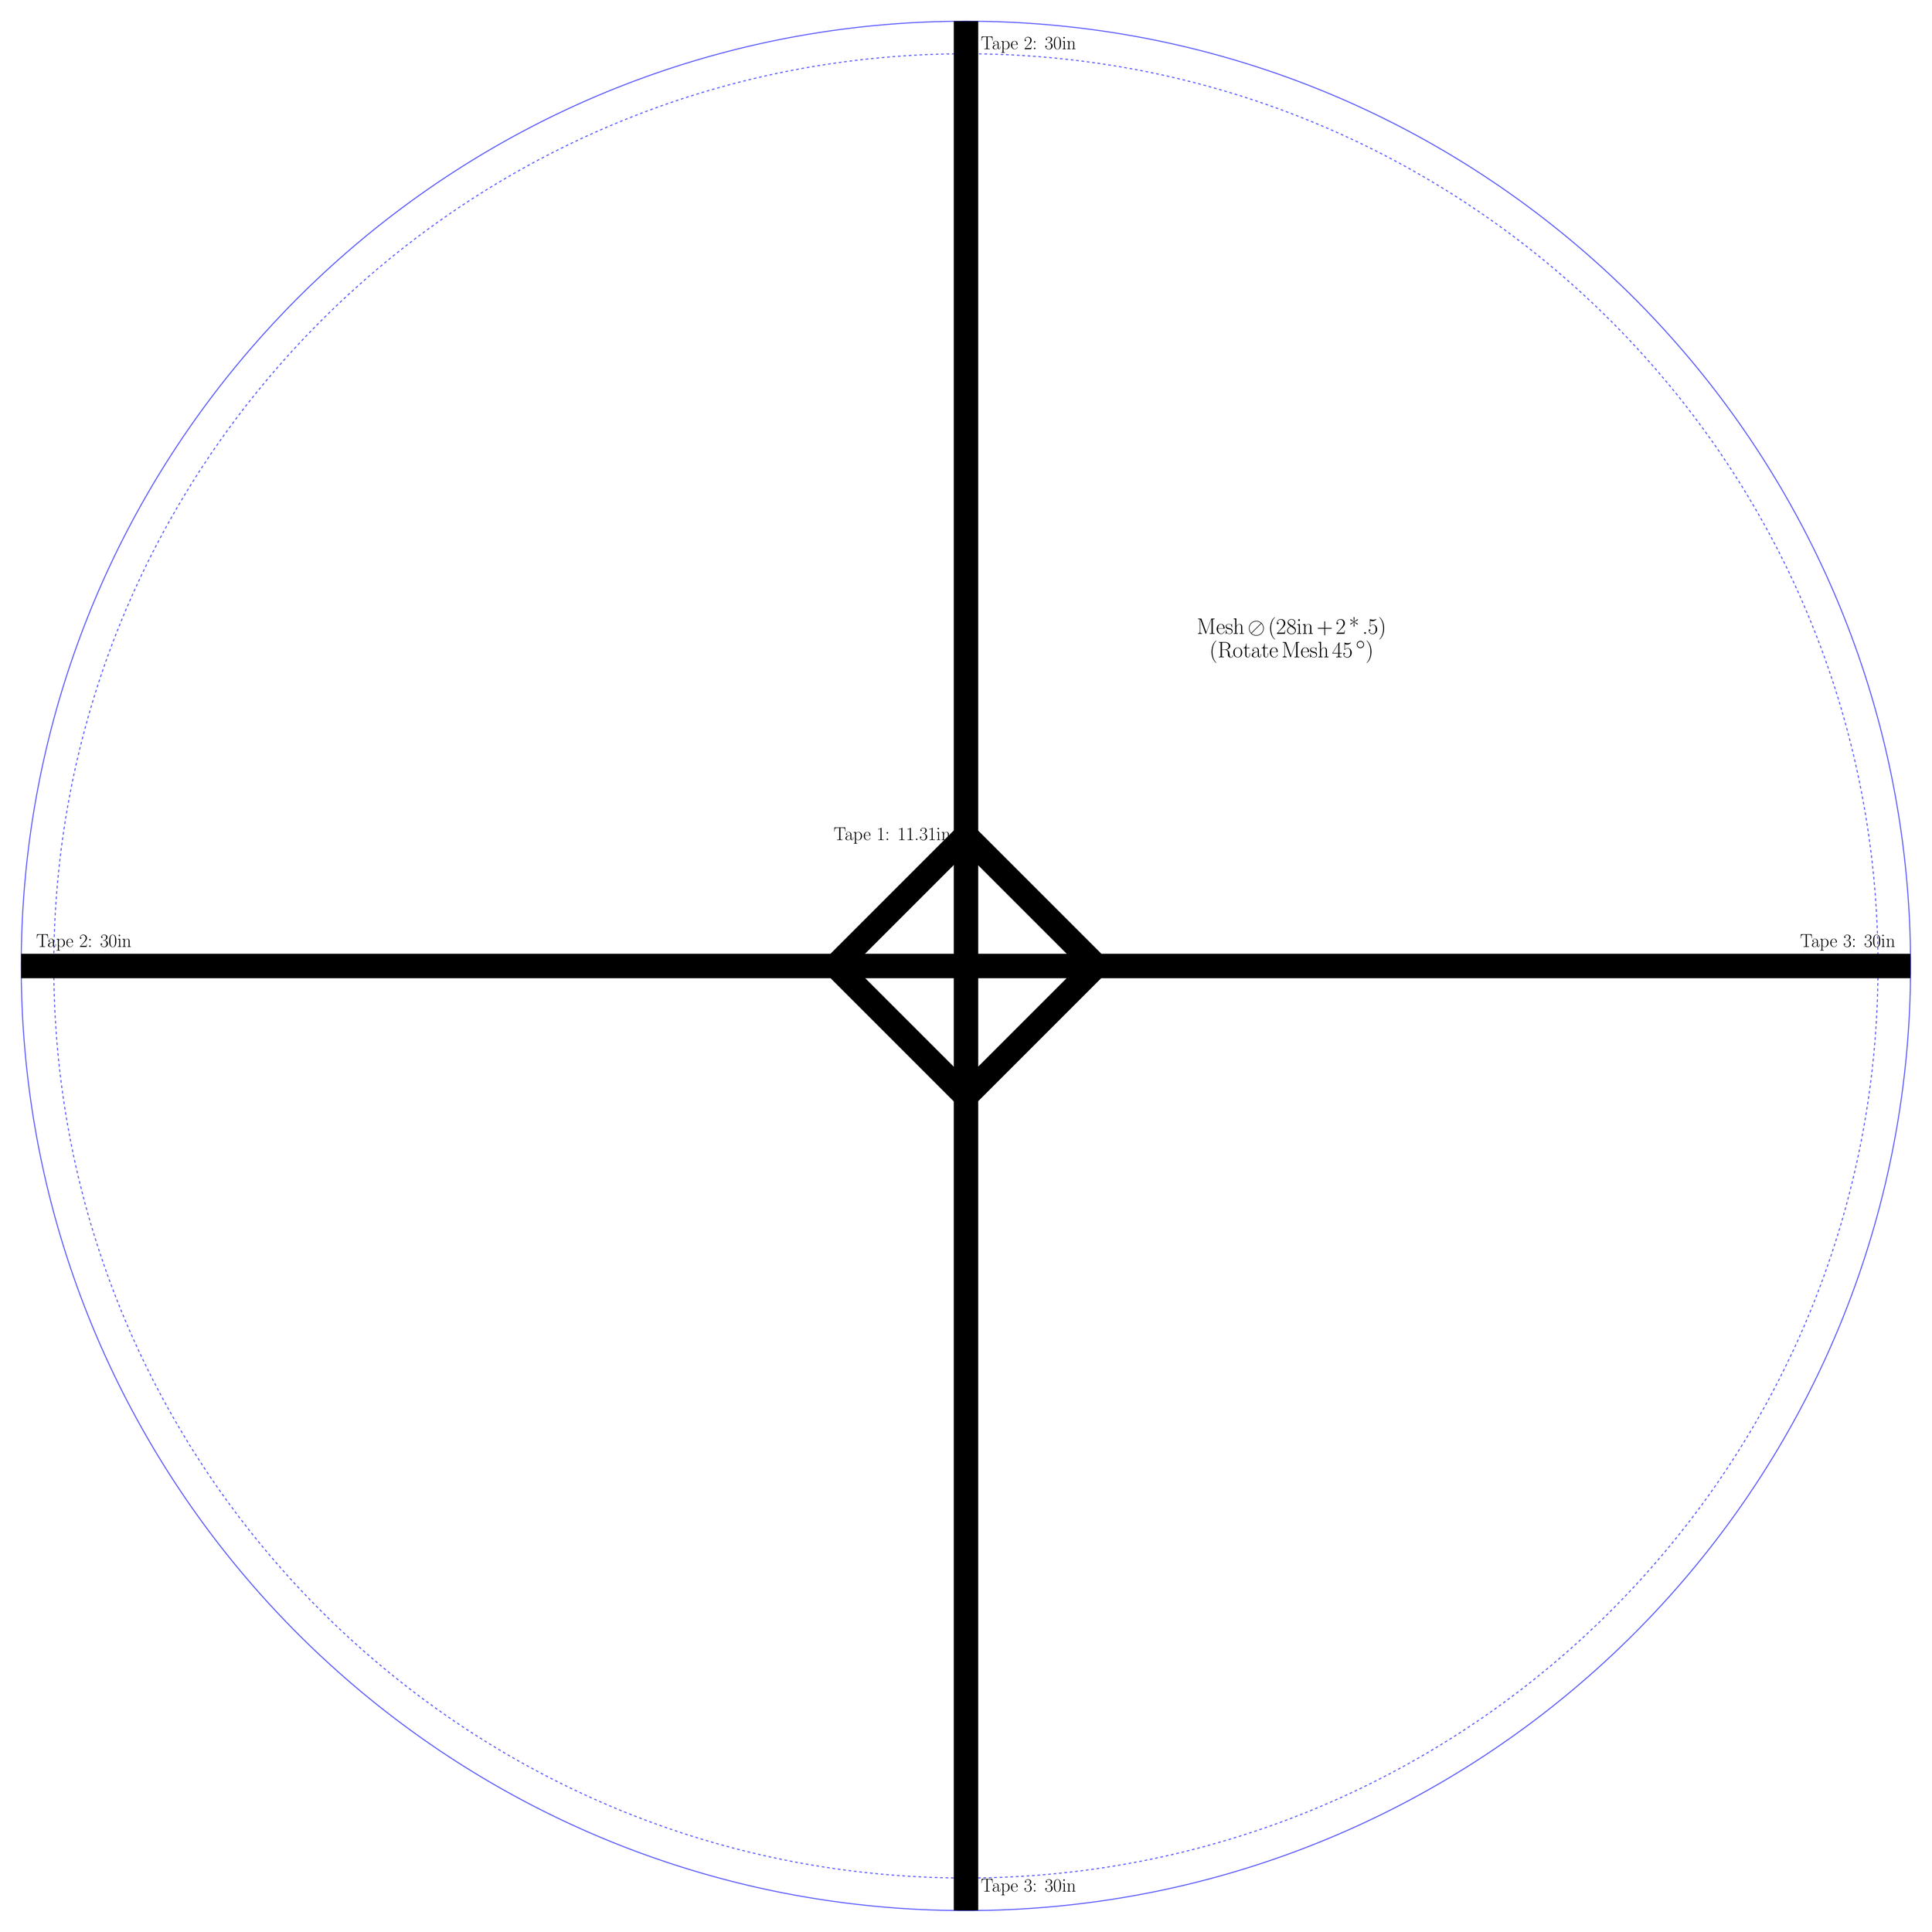
\begin{tikzpicture}[x=1in,y=1in]



\draw[color=blue!60, very thick](0,0) circle (\pcRadOver);
\draw[color=blue!60, very thick, dashed](0,0) circle (\pcrad );
\draw[line width=.375in,black](0,2) -- (2,0) -- (0,-2) -- (-2,0) -- (0,2) node [left] {\huge Tape 1: 11.31in};

\draw[line width=.375in,black](\MpcRadOver,0) node [above right] {\huge Tape 2: \tapeSize in} -- (0,0) -- (0,\pcRadOver) node [below right] {\huge Tape 2: \tapeSize in};

\draw[line width=.375in,black](\pcRadOver,0) node [above left] {\huge Tape 3: \tapeSize in} -- (0,0) -- (0,\MpcRadOver) node [above right] {\huge Tape 3: \tapeSize in};

\node[text width=10in,align=center] at (5,5) {\Huge Mesh $\oslash$ (\pcsize in + 2 * \sewOverlap)  \\ (Rotate Mesh 45 $^{\circ}$)};
\end{tikzpicture}


\end{document}
